This chapter describes X-Project enabling technologies.

The first three sections concern server-side technologies: MongoDB, NodeJS and Loopback by Strongloop (an IBM company).
MongoDB is a NoSQL document-oriented database management system; NodeJS is an event-driven framework to handle Javascript server sides; Loopback is a NodeJS based framework create to use and edit set of APIs.

The fourth, fifth and sixth sections are related to client-side technologies: HTML5, Web Components and Polymer-Project by Google.
HTML5 is a markup language aimed to web pages structuring; Web Components are a set of standards that allow for the creation of reusable widget and components in web documents; Polymer-Project provides a thin layer of API on top of Web Com- ponents and several powerful features, such as custom events and delegation, mixins, accessors and component life-cycle functions, to facilitate the creation of Web Components.

\begin {figure}[h]
\graphicspath{{images/chapter_TCH/}}
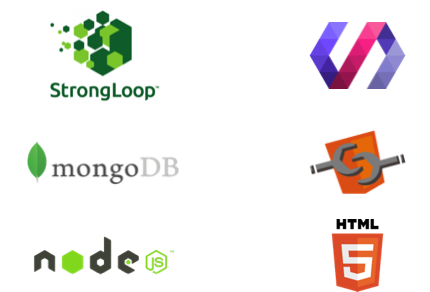
\includegraphics[width=\textwidth]{stack_tch}
\caption{Server and client sides enabling technologies}
\end {figure}
